\begin{figure*}
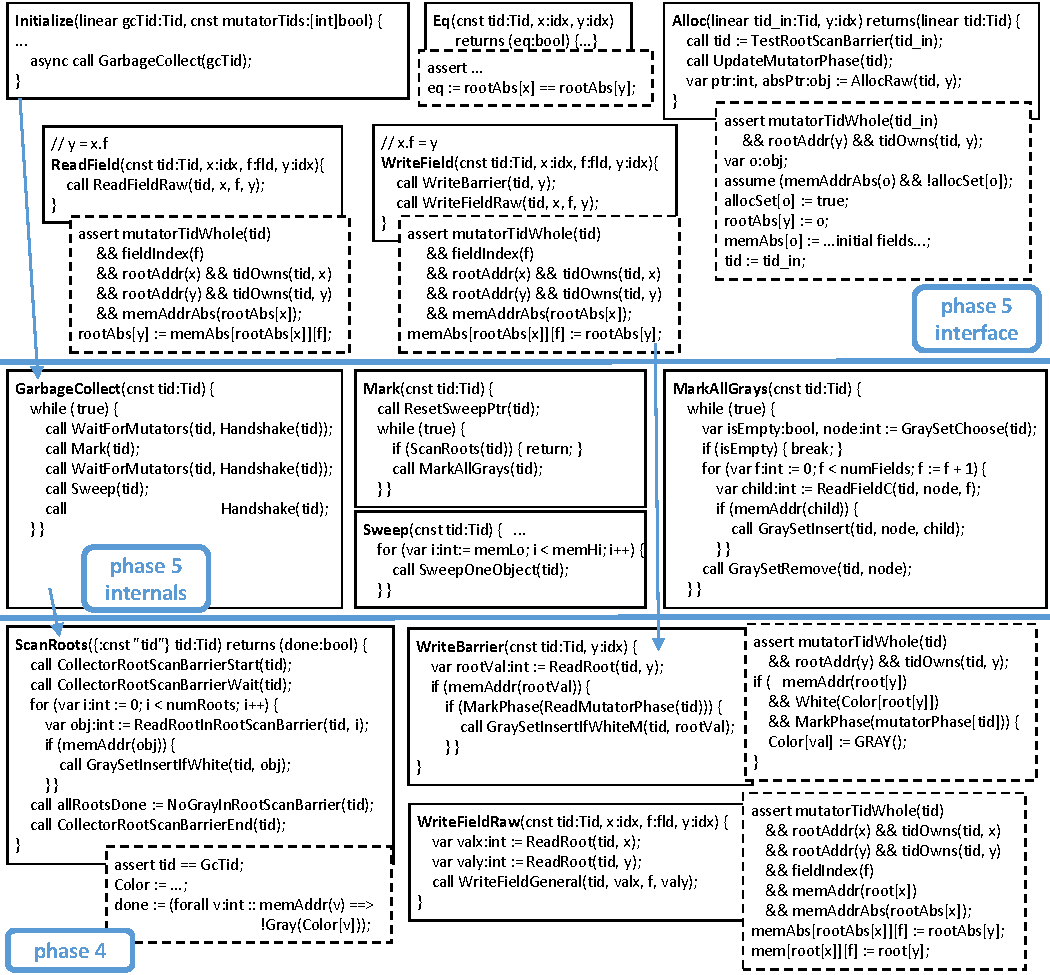
\includegraphics[scale=1.0]{VerifiedGC.pdf}
\caption{Verified garbage collector phases 5, 6 (pseudocode excerpts in solid boxes; atomic action specs in dashed boxes)}
\label{fig:VerifiedGC}
\end{figure*}

We demonstrate the verification methodology and tool on a realistic modern concurrent garbage collector algorithm.
Our algorithm builds on the concurrent collector of Dijkstra et al.~\cite{dijk78}.
Dijkstra's collector is attractive for verification because it maintains a simple tri-color invariant
on the heap objects (in contrast to snapshot-oriented collectors~\cite{doli93,doli94,doma00,azat03}
whose tri-color invariants are more subtle).
By itself, though, Dijkstra's collector is not a modern or performant collector.
First, it becomes incorrect in the presence of more than one program thread (mutator).
Second, it requires that the write-barrier be run not only on updates of heap pointers,
but also on modifications of root pointers, i.e., on modifications of the runtime stacks and the registers;
modern high-performance collectors avoid this overhead.

Therefore, our algorithm (shown inside the solid boxes in Figure~\ref{fig:VerifiedGC}) extends and modifies Dijkstra's collector
to make it work with parallel programs and to not require a write-barrier on root modifications.
Like Dijkstra's collector, our algorithm first {\em marks} all objects reachable from roots (registers and stacks),
shown in Figure~\ref{fig:VerifiedGC}'s Mark procedure, and then {\em sweeps} away all unreached objects,
shown in Figure~\ref{fig:VerifiedGC}'s Sweep procedure.
As in Dijkstra's collector, our algorithm employs a tri-color abstraction to describe the trace of the reachable objects.
Objects are said to be {\em white} if the collector has not seen them yet during the trace.
Objects that the collector encounters become gray and remain gray until the collector scans their children.
Once all the children of an object are noted (meaning that none of them are white), the object becomes black.
The collector works by choosing a node from the set of gray objects (GraySetChoose, called from MarkAllGrays in Figure~\ref{fig:VerifiedGC}),
{\em shading} all its white children to gray (GraySetInsert), and then removing the object from the gray set by making the object black (GraySetRemove).
The shading operation grays a node if it is white, and does nothing otherwise.
The trace terminates when all roots point to black objects (according to ScanRoots)
and there are no more gray objects in the heap (according to IsGraySetEmpty, called by ScanRoots).
Termination is guaranteed because objects can only get darker.
Correctness is guaranteed using an invariant that a black object never points to a white object during the trace
(black objects can only point to gray objects or black objects).
At the end of the trace, objects pointed by the roots must be black, and since no gray objects remain,
black objects only point to black objects,
so the entire set of objects reachable from the roots must be black.

Concurrent mutator operations on objects (ReadField and WriteField in Figure~\ref{fig:VerifiedGC})
could potentially break the no-black-to-white invariant,
because a mutator's WriteField operation could potentially redirect a pointer of a black object to point to a white object.
Therefore, coordination between the program and the concurrent collector is required:
before each raw pointer update (WriteFieldRaw), the WriteField procedure executes a {\em write-barrier} (WriteBarrier).
Before pointer field $x.f$ is set to reference an object $y$,
WriteBarrier shades $y$, ensuring that even if $x$ is black, a pointer from $x$ to $y$
will not violate the no-white-to-black invariant.

The write barrier should shade objects only while the collector is in its mark phase,
not when the collector is sweeping or is idle, and the collector may only switch between phases (mark, sweep, or idle)
when no mutator is in the middle of a WriteField or Alloc operation.
To achieve this (and thereby support correct and efficient support for multiple mutator threads),
we extend Dijkstra's collector with explicit tracking of phases, via a handshaking mechanism~\cite{doli93,doli94}.
A shared variable, collectorPhase, contains the current collector phase.
The collector initiates a handshake by incrementing collectorPhase (in Handshake, called by GarbageCollect).
Each mutator thread keeps cached copy of collectorPhase, and periodically checks to see if
the cached copy mismatches the current collectorPhase, and if so, updates the cached copy
with the most recent value
(in our algorithm, a mutator's call to the allocator, Alloc, checks this in UpdateMutatorPhase,
but the exact location of the check is not critical to correctness).
The GarbageCollector waits until all cached copies equal collectorPhase (WaitForMutators in GarbageCollect),
and then executes a phase (Mark, Sweep, or, for the idle phase, nothing).
Note that each mutator thread can read its own cached phase without acquiring a lock (ReadMutatorPhase in WriteBarrier),
leading to efficient WriteBarrier performance.

Dijkstra's collector requires a write barrier on modifications to roots as well as modifications to objects. 
We eliminate this overhead by employing repeated tracing 
phases until all objects referenced by roots are black. 
A tracing phase starts by stopping all mutators and marking their roots. 
The process of stopping the mutators is similar to a handshake and is done using the CollectorRootScanBarrierStart, CollectorRootScanBarrierWait, and CollectorRootScanBarrierEnd procedures on the collector side and TestRootScanBarrier procedure on the mutator side. 
At the end of the root scan (before the mutators reawaken), all roots point to gray or black objects.
If no gray objects remain (IsGraySetEmpty), then all roots point to black objects, and marking is complete. 
Otherwise, we trace from gray objects until completion and start a new
tracing phase (by stopping the mutators and checking the roots again). 
In a worst-case theoretical scenario we may need to run many root scans and discover more and more white root descendants to trace each time. 
But in practice we usually finish after a small number of scans,
so we obtain correctness and termination in all scenarios and we obtain good performance in real-world scenarios. 



